\section{ChatCoT}
\subsection{现有方法}
\begin{frame}{Tool}
    利用外部工具的方法可以大致分为以下两类:
    \begin{enumerate}
        \item \textbf{模型参数微调} \\
        这一类方法(如 Gao et al., 2023;Parisi et al., 2022;Qiao et al., 2023)通过训练模型参数来支持外部工具的集成与使用。这通常需要收集或生成工具增强示例以用于模型参数微调(如 Schick et al., 2023;Patil et al., 2023;Hao et al., 2023)。
        \pause
        \item \textbf{基于提示的工具指导} \\
        第二类方法(如 Gao et al., 2022;Yao et al., 2022;Zhang et al., 2023)主要依靠设计提示(prompts)来引导大型语言模型(LLMs)使用外部工具。这些方法重点在于设计合适的提示或工具操作策略,以便在需要时选择和使用工具(如 Liang et al., 2023;Shen et al., 2023;Yao et al., 2022)。
    \end{enumerate}
    
    文章采用了第二种方法。
\end{frame}


\begin{frame}{链式推理(Chain-of-Thought, CoT)}
    \textbf{链式推理(CoT)}提示策略(Wei et al., 2022; Kojima et al., 2022)旨在通过引导大型语言模型(LLMs)生成中间推理步骤来增强其推理能力。这种方法通过两种主要机制实现:
    \begin{enumerate}
        \item \textbf{特殊指令}:例如 "Let us think step by step",直接引导模型输出分步骤的推理过程。
        \item \textbf{上下文示例}:提供详细的、包含中间推理步骤的示例,帮助模型从类似问题中学习逐步推理的方法。
    \end{enumerate}
    
    通过上述策略,LLMs 能够依次进行每个推理步骤,直到得出最终答案,显著提升整体性能。
\end{frame}

\subsection{基于 CoT 的改进研究}

\begin{frame}{基于 CoT 的改进研究}
    近年来,基于 CoT 的方法被进一步优化,以改进其推理性能,主要包括以下几个方向:
    \begin{itemize}
        \item \textbf{问题分解}:将复杂问题拆解为多个子问题,逐步解决后组合答案(Zhou et al., 2022; Dua et al., 2022)。
        \item \textbf{示例选择}:选择更恰当、更具代表性的上下文示例以指导推理(Ye et al., 2022; Shi et al., 2023)。
        \item \textbf{结果后处理}:在生成答案后通过后处理减少错误或调整输出(Wang et al., 2022; Madaan et al., 2023; Zheng et al., 2023)。
        \item \textbf{推理格式变更}:尝试修改推理格式或流程以提升模型理解和输出的准确性(Yao et al., 2023; Wu et al., 2023)。
    \end{itemize}
\end{frame}

\begin{frame}{现存问题与改进方向}
    尽管链式推理方法取得了显著进展,但其生成过程通常为\textbf{一次性完成(one-pass generation)},这意味着模型从问题到答案的推理流程是自上而下的连续生成。若在中间步骤需要使用外部工具(如计算器、检索系统等),可能会中断推理的流畅性,影响生成效果。
    % \bigskip
    
    为了解决这一问题,作者提出了一种\textbf{将链式推理与工具操作无缝结合的统一方法}。利用大型语言模型在多轮对话中的强大能力,设计了基于多轮对话的链式推理策略,能够在不同步骤灵活调用工具的同时,保持推理过程的连贯性,从而更好地解决复杂问题。
\end{frame}


\subsection{工具操作 (Tool Manipulation)}

\begin{frame}{工具操作 (Tool Manipulation)}
    大型语言模型(LLMs)在处理算术计算时比较困难,而这些问题可以通过使用特定的外部工具(如计算器)解决。这些外部工具被表示为 $\{T_1, \dots, T_n\}$。为操作工具,现有方法主要依赖编写详细的 prompt ,描述如何让 LLM 使用这些工具。具体流程为:
    \begin{enumerate}
        \item 编写提示以指导 LLM 选择有用的工具;
        \item 生成工具的参数输入;
        \item 调用工具的 API 获取结果。
    \end{enumerate}
\end{frame}
\begin{frame}{工具操作 (Tool Manipulation)}  
    作者延续了这一思路,主要使用三种工具:
    \begin{enumerate}
        \item \textbf{计算器(Calculator)}:给定数学表达式,计算器可以根据算术规则(如合并同类项、化简分数)计算表达式的值或进行化简。
        \item \textbf{方程求解器(Equation Solver)}:给定方程组和未知变量,方程求解器可以利用相关算法计算未知变量的值。
        \item \textbf{检索器(Retriever)}:给定查询,检索器旨在从候选集中提取最相关的信息(如文档)。根据检索语料的类型,可以通过专门的模型(如密集检索模型)实现。
    \end{enumerate}
\end{frame}

\begin{frame}{实现方法}
    \begin{itemize}
        \item \textbf{计算器与方程求解器}:使用 Python 符号计算库 SymPy(Meurer et al., 2017)中的不同函数实现 Calculator 和 Equation Solver 工具。
        \item \textbf{检索器}:采用 SimCSE(Gao et al., 2021)句子嵌入模型来计算文本语义相似性,利用该方法检索出语义上最相似的前 $k$ 个示例,并将这些示例的问题描述 $Q$ 和解决方案 $S$ 拼接起来,作为输入提示。同时将期望的回答一并输入到大型语言模型中。
    \end{itemize}
    
    当输入的表达式或方程格式不正确(ill-formed)或无法求解时,以上工具都会返回错误结果。
\end{frame}

\subsection{现有的两种工具增强方法的缺点}

\begin{frame}{现有的两种工具增强方法的缺点}
    这两种工具增强方法各自存在一些潜在的问题:

        \textbf{依赖大型语言模型 (LLM) 预先安排工具使用计划并在随后执行的方法}(Zhou et al., 2022; Jiang et al., 2023b)无法在生成计划后与工具交互,即使发现明显的错误也无法修正。
        
        \pause
        这种方法将工具的使用视为一个独立于推理过程的步骤,LLM 首先要规划好所有需要使用的工具以及它们的调用顺序,然后才开始执行计划。这种方式的缺点在于,LLM 在规划阶段无法预知推理过程中可能出现的各种情况,因此计划很容易出现错误。并且,由于计划和执行是分离的,LLM 在执行过程中即使发现计划有误也无法进行调整,只能继续执行错误的计划,最终导致推理结果出错。
\end{frame}    
\begin{frame}{现有的两种工具增强方法的缺点}    
        \textbf{需要针对特定任务设计形式化动作的方法}(Dua et al., 2022; Khattab et al., 2022; Jiang et al., 2023a)必须频繁地在 LLM 推理和执行动作之间切换,这会损害 CoT 推理过程的连续性。
        
        \pause
        这种方法将工具的使用融入到推理过程中,LLM 在推理的每一步都需要决定是否使用工具,以及使用哪个工具。这种方式的缺点在于,LLM 需要频繁地在推理和工具使用之间切换,这会打断推理的思路,降低推理的效率。并且,由于每个工具都需要设计特定的动作,这种方法的可扩展性较差,难以应用于新的工具或新的任务。
        
        \pause
    总的来说,这两种方法都试图将外部工具与 LLM 结合起来以解决复杂推理任务,但在如何协调工具使用和推理过程方面存在不足。前者缺乏灵活性,后者缺乏效率。
\end{frame}

% Section: ChatCoT Framework
\subsection{ChatCoT框架的工作原理}

\begin{frame}{ChatCoT框架的工作原理}
    \textbf{ChatCoT框架的工作原理}:
    \begin{enumerate}
        \item \textbf{在对话的早期阶段提供背景知识}。例如工具描述、相关任务示例和聊天中分解思维链的演示。例如 "\([T]\) can help you \([Y]\)", 其中 \([T]\) 是工具名称,\([Y]\) 显示其详细功能。然后把这些描述作为输入提示。
        \pause
        \item \textbf{将思维链推理过程分解为多轮对话}。从训练集中随机抽取五个问题,并手动标注这些问题的完整多轮对话作为示例。然后将所有示例的对话逐轮输入到对话的 prompt 中,作为\textbf{上下文}来引导 LLM 遵循该格式进行推理。
        \pause
        \item \textbf{使用工具增强推理步骤,以逐步执行推理,直到获得最终答案}。在每个迭代中,大型语言模型执行推理,选择适当的工具,并执行所选工具以获得当前步骤的中间结果。
    \end{enumerate}
\end{frame}   

\begin{frame}{ChatCoT框架的工作原理}
    \begin{figure}
        \centering
        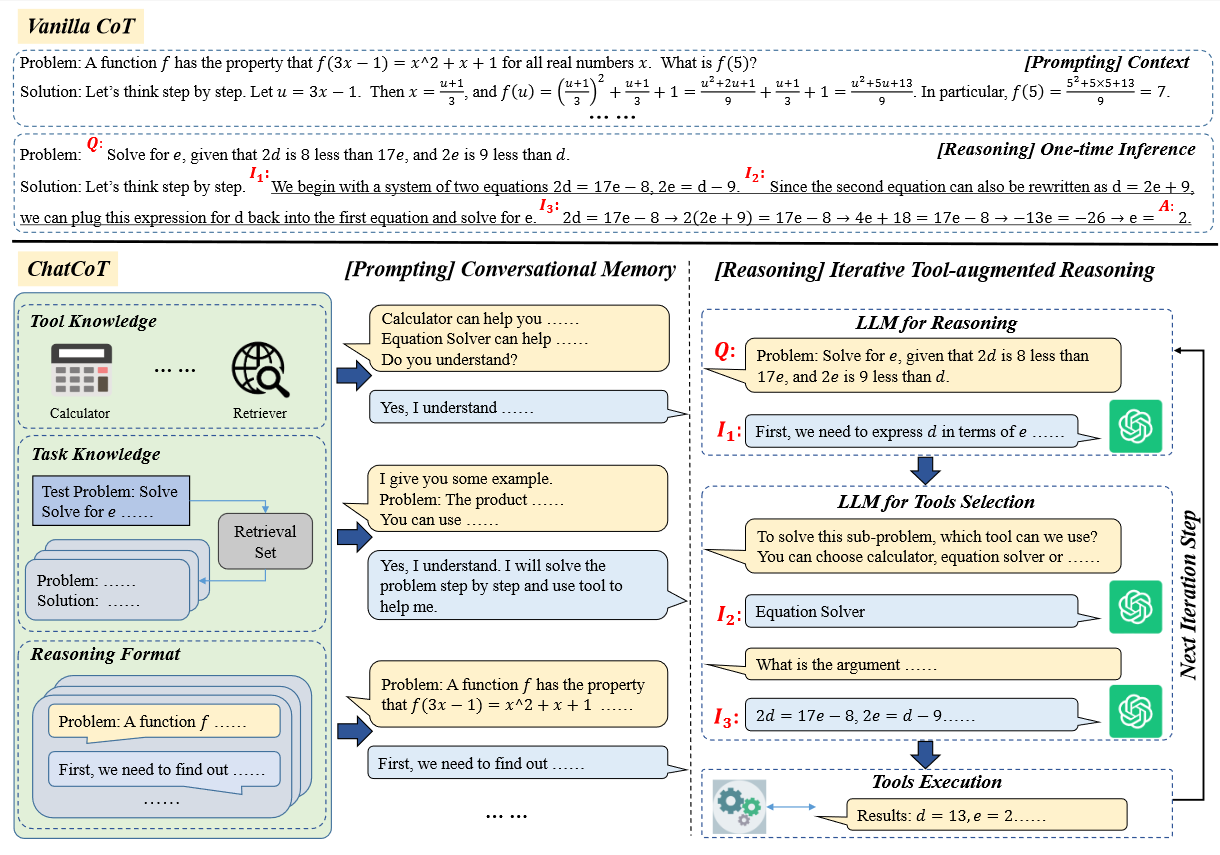
\includegraphics[width=.6\linewidth]{./pic/vanilla_CoT_and_ChatCoT.png}
        \caption{ChatCoT架构示意图}
        \label{fig:chatcot}
    \end{figure}
\end{frame}

\begin{frame}{举例}
    \textbf{Tool Knowledge}
    
    The two-turn utterances are:
    
    \textbf{User}: \\
    “You can use tool to help you solve the problem and I give you the instruction of tools usage. 
    \( T_1 \) can help you \( Y_1 \) · · · Do you understand?”
    
    \textbf{LLM}: \\
    “Yes, I understand. I will use tool to help me solve the problem.”
    
    % \bigskip
\end{frame}
\begin{frame}{举例}   
    \textbf{Retrieval-Augmented Task Knowledge}
    
    The two-turn utterances are:
    
    \textbf{User}: \\
    “I give you some examples. 
    Problem: \( Q_1 \)  
    Solution: \( S_1 \)  
    · · · 
    You can use the knowledge and theory in these problems. Do you understand?”
    
    \textbf{LLM}: \\
    “Yes, I understand. I will solve the problem step by step and use tool to help me.”
    
    % \bigskip
\end{frame}
\begin{frame}{举例}
    
    \textbf{Multi-turn Reasoning Format}
    
    The multi-turn utterances are based on the following pattern:
    
    \textbf{User}: \\
    “Problem: \( Q'_1 \)  
    Let’s think step by step and use knowledge in similar problems to solve this problem.”
    
    \textbf{LLM}: \\
    “\( I_1 \)”  
    ... 
    “\( I_n \)”
\end{frame}

% Section: LLMs Reasoning and Tool Selection
\subsection{LLMs 推理与工具选择}

\begin{frame}{LLMs 推理(LLM for Reasoning)}
    LLMs 借助上下文中的示例直接用自然语言进行推理,直到需要工具的功能来推动解决任务。
\end{frame}

\begin{frame}{LLMs 工具选择(LLM for Tools Selection)}
    在完成推理之后,利用 LLM 来选择合适的工具(如计算器)以提供所需的功能。输入给 LLM 的提示是:
    
    \textit{"解决这个子问题,我们可以使用哪个工具?"}
    
    模型根据该提示判断是否需要使用工具:
    \begin{itemize}
        \item 如果需要使用工具,模型会选择一个合适的工具,并进一步生成工具的输入参数,例如数学表达式。
        \item 如果不需要工具,模型直接回答“Do not use tool”,并继续进行推理。
    \end{itemize}
\end{frame}

\begin{frame}{工具执行(Tools Execution)}
    基于 LLM 所选择的工具和生成的输入参数,使用该工具并以参数执行计算或任务,获取当前迭代结果。再由 LLM 判断结果是否符合预期,如果不符合预期可以重复执行工具。
    
    
    \textbf{问题:} 由 LLM 判断结果是否符合预期?这种验证是否缺乏说服力和可信度?
\end{frame}